\documentclass[ngerman,11pt]{article}
\RequirePackage{latex_basic_head}
\addbibresource{441.bib}
\usepackage{geometry}
\geometry{a4paper,left=1cm,right=1cm,top=1cm,bottom=1.5cm}
\usepackage{multicol}
\newcommand{\kin}{\mathrm{kin}}
\newcommand{\ug}{U_{0}}
\title{Versuch 441 Weißlichtspektroskopie an Gold-Nanostrukturen}
\author{Wenjie Wu,~Lars }
\date{\today}
\begin{document}
	\maketitle
	\begin{abstract}

	\end{abstract}
	\begin{multicols}{2}
		\section{Einleitung}
		Ziel dieses Versuchs ist es, sich mit der Detektion von $\gamma$-Spektrum. Dazu wird zwei Detektoren benutzen: Szintillationsspektrometer und  Halbleiterdetektor.
		\section{Theorie}
		\subsection{Radioaktiver Zerfall}
		Ionisierende Strahlung stammt entweder aus natürlicher Umwelt oder aus künstlichen Strahlungsquellen. Die primäre Strahlung besteht aus massiven geladenen Teilchen oder aus masselosen neutralen Quanten wie Photonen oder Neutrinos. Die Strahlung aus der natürlichen Umwelt stammt aus zwei verschiedenen Quellen: die eine ist die kosmische und solare Teilchenstrahlung, die andere ist die natürliche Radioaktivität. Dabei entsteht $\alpha$-, $\beta$-, oder $\gamma$-Strahlung, die jeweils aus dem radioaktiven Zerfall $\alpha$-, $\beta$-, oder $\gamma$-Zerfall kommt. Überwiegend in diesem Versuch ist der $\gamma$-Zerfall, welche Reaktionsgleichung besagt:
		\[
		^A_ZX^*_N\rightarrow ^A_ZX_N+\gamma
		\] 
		Die instabile Kerne kann durch mehrere radioaktive Zerfälle in den stabilen Zustand kommen, das ist sogenannte Zerfallsreihen.
		\subsection{Wechselwirkung von $\gamma$-Photon mit Matrie}
		Strahlung kann auf verschiedene Arten mit Materie wechselwirken. Folgende Prozesse sind die M\"oglichkeiten:
		\paragraph{Compton-Effekt} 
		Nach die Teilchen-Wellen-Dualismus, das Photon kann als Teilchen mit Materie wechselwirken. Bein Compton-Effekt wird das Photon von einem Elektron in der Atom gestreut. Dabei \"ubertr\"agt das Photon einen Teil seiner Energie an das Elektron und die Wellenl\"anger der einfallenden Strahlung vergr\"o\ss ert sich.
		\paragraph{Photoeffekt}
		Beim Photoeffekt l\"ost das Photon ein Elektron aus. Das gel\"oste Elektron hat die kinetische Energie von der Energie des Photon. Um das Photoeffekt zu passiert, muss das Photon hat die Energie gr\"o\ss er als die Austrittsarbeit.
		\paragraph{Paarbildung}
		Wenn die Energie des Photons gr\"o\ss er als die Ruheenergie eines Elektron-Positron-Paars($e^+$-$e^-$-Paar) ist, kann aus dem Photon ein $e^+$-$e^-$-Paar erzeugen. Damit wird $e^+$-$e^-$-Paar weiter mit Materie(Detektor) wechselwirken, und das Photon existiert nicht mehr.
		\paragraph{Wirkungsquerschnitt}
		Die Wirkungsquerschnitten von verschiedener Wechselwirkungen sind nicht gleich. Die Abh\"angigkeit des Wirkungsquerschnittes von der Energie das Photon $E_{\gamma}$ und der Ordnungszahl $Z$ des Absorbermaterials lauten:
		\begin{center}
			\centering
			\begin{tabular}{|c|c|}
				\hline 
				Effekte & Proportionalit\"aten \\ 
				\hline 
				Compton-Effekt & $\propto ZE_\gamma^{-1}$ \\ 
				\hline 
				Photoeffekt & $\propto Z^5E_\gamma^{-\frac{7}{2}}$, für $ E_\gamma<m_ec^2$.\protect \footnotemark[1]\\ 
				\hline 
				Paarbildung & $\propto Z^2\ln{E_\gamma}$ \\ 
				\hline 
			\end{tabular} 
		\end{center} 
	\footnotetext[1]{In diesem Versuch wird nur an diese Bedingung betrachtet.}
		Die gesamt Wechselwirkung ist die Summe der Wirkungsquerschnitten von verschiedenen Wechselwirkungen. 
		\subsection{Szintillationsspektrometer und Halbleiterdetektor}
		Ein Szintillationsspektrometer (Abb. \ref{szintillator})\footnote[2]{\url{https://de.wikibooks.org/wiki/Physikalische_Grundlagen_der_Nuklearmedizin/_Szintillationszähler}} nutzt aus, dass bei einige Materialien Licht entsteht, wenn diese mit Teilchen oder Photonen bestrahlt werden. Mit Hilfe eines Photomultipliers wird dieses Signal in ein elektrisches Signal umgewandelt.
		\begin{figure}[H]
			\centering
			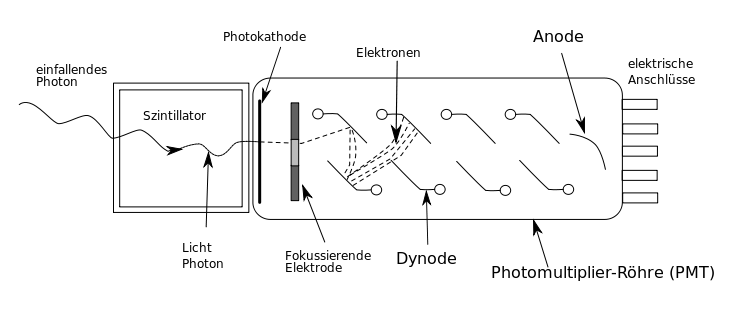
\includegraphics[width=0.45\textwidth]{szintillator.png}
			\caption{Schematischer Aufbau eines Szintillator mit Photomultiplier}
			\label{szintillator}
		\end{figure}
		\paragraph{Szintillator}
		Hier wird einen anorganischen Szintillator verwendet, in dem die Prozesse durch das Bändermodell beschrieben werden können. Das Elektron wird entweder von der Strahlung vom Valenzband ins Leitungsband angeregt, sodass ein freies Elektron und ein Loch entstehen. Wenn das Elektron ins Valenzband zur\"uckfallen, wird dann Photon emittiert. Die Energiedifferenz zwischen Valenzband und Leitungsband ist zu gro\ss, sodass das emittierte Photon nicht in sichtbar Bereich legen. Wenn das Szintillator mit andere Atom dotiert, gibt es noch Exzitionband zwischen Valenzband und Leitungsband. Wenn das Elektron ins Exzitionband fallen, das emittierte Photon hat ein Wellenl\"ange in sichtbar Bereich. Das emittiert Photon(in sichtbar Bereich) kann durch Photomultiplier detektiert werden.
		\paragraph{Photomultiplier}
		Im Photomultiplier treffen die Photonen auf die Photokathode. Hier wird mittels des Photoeffekts ein freies Elektron erzeugt. Diese wird von der Dynode beschleunigt. Beim Auftreffen auf die Dynode überträgt das Elektron seine Energie an andere Elektroden, sodass weitere freie Elektronen entstehen. Dieser Prozess wiederholt sich an jeder Dynode, sodass immer mehr Elektronen beschleunigt werden. Zum Schluss werden alle Elektronen von der Anode aufgenommen und erzeugen einen Strom. 
		\paragraph{Halbleiterdetektor}
		Die Halbleiterdetektoren sind meist als dünne Halbleiterplättchen, die einen pn-Übergang enthalten, in der Sperrrichtung ausgebildet. Ionisierende Strahlung erzeugt darin Paare von Elektronen und Löchern, und zwar mit viel geringerem Energieaufwand als für die Ionisierung eines Gasmoleküls. Die im rein p- oder rein n-leitenden Bereich erzeugten Paare rekombinieren bald wieder. In der pn-PBergangsschicht aber werden Elektronen und Löcher durch das dort herrschende starke Raumladungsfeld getrennt. Je größer die äußere Sperrspannung liegt, desto dicker ist die Zone. \cite{gerthsen}
		Zur Detektion von $\gamma$-Strahlung wird Germanium aufgrund seiner höheren Massenzahl gegenüber Silizium bevorzugt. Wegen der kleineren Bandlücke ist jedoch der Leckstrom in Germanium bei normalen Temperaturen zu hoch, muss den Halbleiterdetektor von flüssigem Stickstoff gekühlt werden. 
		\paragraph{Vergleich von Szintillations- und Halbleiterdetektor}
		Die Bandl\"ucke im Halbleiter ist wesentlich kleiner als die im Kristall des Szintillators. Deswegen bietet der Halbleiterdetektor eine h\"ohere Energieaufl\"osung. Das Szintillator kann gro\ss sein. Deswegen kann das Szintillationsdetektor mehr Photon aufnehmen. Beispielhaft wird die
		 Gamma-Spektroskopie in der Abb. \ref{aufloesung} dargestellt. Man kann deutlich die geringere Energieaufl\"osung des Szintillationsdetektors erkennen.
		\begin{figure}[H]
			\centering
			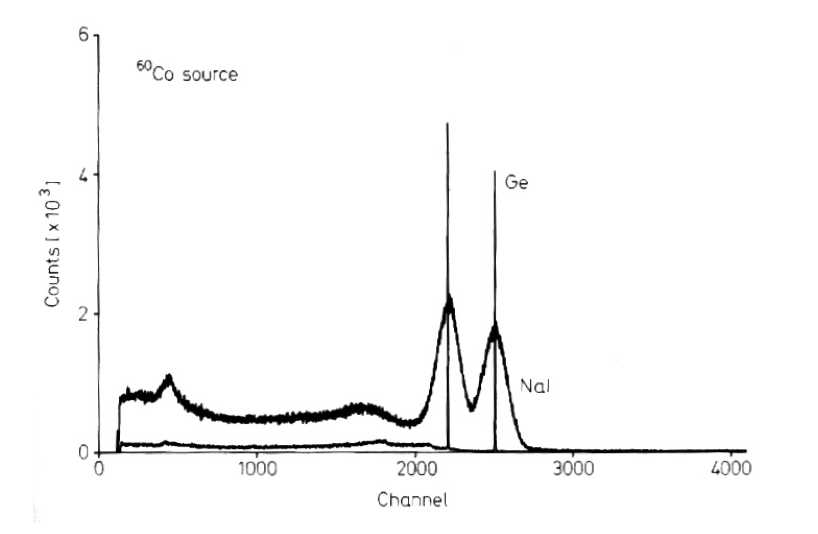
\includegraphics[width=0.45\textwidth]{aufloesung.png}
			\caption{Gammalinien der beiden Detektoren. \cite{techniques}}
			\label{aufloesung}
		\end{figure} 
		\subsection{Impulshöhenspektrum}

		\begin{figure}[H]
			\centering
			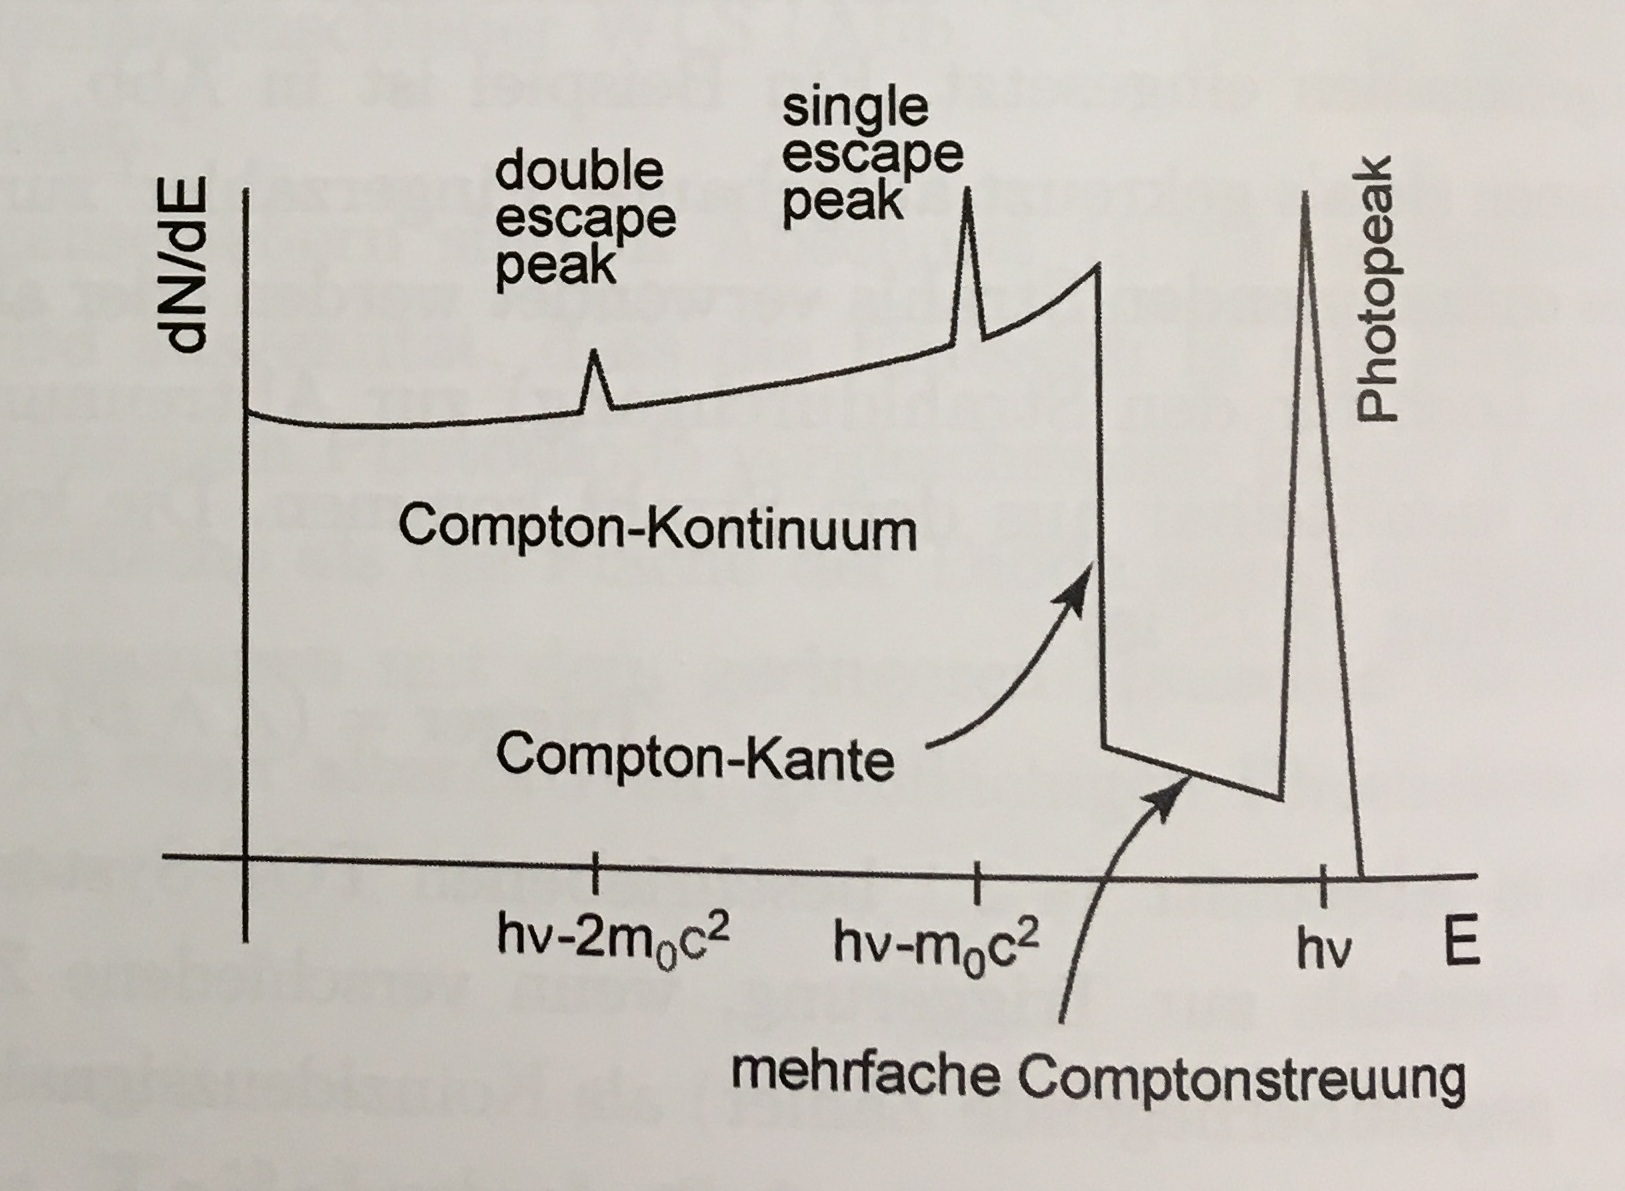
\includegraphics[width=.5\textwidth]{spektrum1.jpg}
			\caption{Energiespektrum eines Szintillators \cite{teilchen}}
			\label{spektrum}
		\end{figure}

		Die Abbildung (\ref{spektrum}) zeigt schematisch das Energiespektrum eines Szintillators. Es lassen sich drei charakteristischen Merkmale erkennen. Diese sind in der Reihenfolge der für den erzeugenden Effekt benötigten Energie aufgezählt.
		\paragraph{Photopeak}
		Dieser Peak entsteht durch die Absorption eines Photons und das dadurch emittierte Elektron. Dieses Elektron spiegelt die Gesamtenergie der einfallenden $\gamma$-Strahlung wieder. Dieses Elektron wiederum ionisiert das Szintillator-Material und führt zur Emission eines Photons.
		\paragraph{Compton-Kante}
		Die Compton-Kante und das Compton-Kontinuum lassen sich auf die Wechselwirkung zwischen Photon und dem Szintillator durch den Compton-Effekt zurückführen. Bei diesem Effekt gibt das Photon nicht seine gesamte Energie an das Elektron weiter. Dem entsprechend findet man die Compton-Kante bei einer geringeren Energie als den Photopeak. Das Maximum des Compton-Kontinuums befindet sich bei einem Streuwinkel von 180$^\circ$. Dieser sogenannte Rückstreupeak ist in der Abbildung (\ref{spektrum}) allerdings nicht vorhanden.
		\paragraph{Escape Peaks}
		Bei diesem Peak ist die Paarbildung von entscheidender Rolle. Das so erzeugte Positron verbindet sich anschließend mit einem Kristall Elektron. Hierbei entstehen zwei Photonen von denen eines (single escape peak) oder beide (double escape peak) vom Detektor registriert werden können.
		\paragraph{Rückstreupeak}
		Die Photonen, die durch die Materie ohne Wechselwirkung passieren, werden mit verringerter Energie in den Szintillator zurückgestreut. Trifft das Photon nach einer Streuung um ungefähr 180$^{\circ}$ auf den Photomultiplier, so erzeugt es ein Signal bei $E_{rück}=E_\gamma-E_{max}$.

		\subsubsection{Vielkanalanalysatoren (MCA)}

		Ein Vielkanalanalysator (\textit{Multi Channel Analyzer}) zählt Impulse innerhalb verschiedener Amplitudenintervalle. Die Signale werden mit einem Analog-Digital-Wandler digitalisiert,  die als Adresse eines Speicherplätze fungieren und bei jedem Zugriff den Zählerstand erhöht. Das Ergebnis dieser Zählweise ist ein Histogramm. Durch eine Energiekalibration kann den Kanalen ein Energieintervall zugeordnet und das Histogramm representiert das Energiespektrum. \cite{messelektronik}

		\subsection{Eigenschaften des Detektors}

		\paragraph{Peak-to-Total-Verhältnis}
		Diese Größe gibt an, welcher Anteil der im Detektor registrierten  $\gamma$-Quanten eines bestimmten Übergangs im Photopeak enthalten sind. Die Definition des Peak-to-Total-Verhältnis lautet:
		\[
		\dfrac{\text{Anzahl des Ergebnis~im~Photonpeak}}{\text{Gesamtzahl~aller Ergebnisse~im~Spektrum}}
		\]
		\paragraph{Absolute Peakeffizienz}
		Zur Kalibrierung der Effizienz der photoelektrische Umwandlung benötigt die absolute Peakeffizienz: \cite{techniques}
		\[
		\dfrac{\text{gesamte Zählrate im Photopeak}}{\text{gesamte Zählrate im Detektor}}
		\]
		\textbf{Nachweiswahrscheinlichkeit(Efficiency)}\\
		Bei der allgemeinen Diskussion werden zwei Arten von Efficiency genannt: Die absolute Nachweiswahrscheinlichkeit $\epsilon$ und die interne Nachweiswahrscheinlichkeit $\epsilon_i$. Die absolute Nachweiswahrscheinlichkeit ist definiert als: \cite{techniques}

		\[
		\frac{\text{Teilchen im Detektor registriert}}{\text{Teilchen aus Quelle emmitiert}}
		\]

		\subsection{Termschemata}
		F\"ur diesen Versuch werden drei verschiedene Quellen verwendet, die Zerfallsschemata werden in Abb.(\ref{fig:coterm})(\ref{fig:csterm}) (\ref{fig:euterm}) dargestellt.
		\begin{figure}[H]
			\centering
			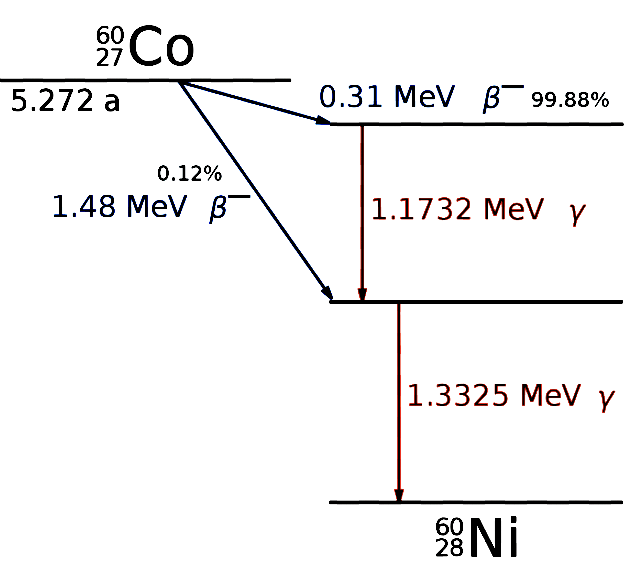
\includegraphics[width=0.3\textwidth]{coschema.png}
			\caption{Termschema des $^{60}$Co-Zerfalls. \protect\footnotemark[1]}
			\label{fig:coterm}
		\end{figure}
		\begin{figure}[H]
			\centering
			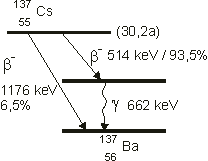
\includegraphics[width=0.3\textwidth]{csschema.png}
			\caption{Termschema des $^{137}$Cs-Zerfalls. \protect\footnotemark[2]}
			\label{fig:csterm}
		\end{figure}

		\begin{figure}[H]
			\centering
			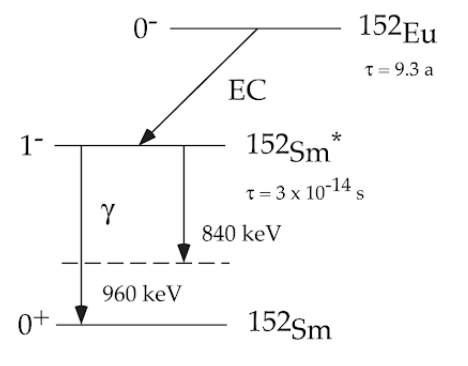
\includegraphics[width=0.3\textwidth]{euterm.png}
			\caption{Termschema des $^{152}$Eu-Zerfalls\cite{kern}}
			\label{fig:euterm}
		\end{figure}

		\footnotetext[1]{\url{https://de.wikipedia.org/wiki/Zerfallsschema}}
		\footnotetext[2]{\url{http://archive.is/XAO5R}}
		\section{Aufbau}
		Der Versuchsaufbau wird in Abb.[fig] dargestellt. Die wesentlischen verwendeten Bauteile waren die Detektoren mit Vorverst\"arker, der Hauptverst\"arker und der Computer mit der Software MCDWIN. Man kann die Detektoren w\"ahlen. Es gab zwei verschiedene Detektoren: Germanium-Detektor(Halbleiterdetektor) und Szintillationsdetektor. Die Probe befand sich im Abstand $d$ zum Detektor.
		\section{Durchf\"uhrung}
		[wait lars]
		\section{Auswertung}
		\subsection{Energiekalibrierung}
		Als erstes wurde nun eine Energiekalibrierung beider Detektoren vorgenommen. Dazu werde die Spektren von verschiedene Quellen und Detektoren minus die Untergrunde angetragen (siehe Abbildung (\ref{fig:spektrummunusunter})). Die Fehlers werden berechnet durch Gau\ss-Fehlerfortpflanzen. Dann werden verschiedene bekannte Energielinien mit Hilfe von Gau\ss-Kurven an die Daten angepasst:
		$$
		f(x) = A\cdot\exp\left( -\ln(2)\cdot\frac{(x-\mu)^2}{\mathrm{HWHM}^2} \right)
		$$
		$A$ ist die Amplitude der Kurve, $\mu$ ist der Mittelwert und HWHM ist half Bereite am half Maximum (also HWHM = $\sqrt{2\ln2}\sigma$, mit Standortabweichung $\sigma$ ). Diese Kurve ist kein klassische Gau\ss-Kurve, aber mit HWHM kann man einfach FWHM bestimmen, das ist f\"ur weitere Auswertung gut. Die Ergebnissen f\"ur diese Kurve-Anpassung siehe Tabelle (\ref{tab:gefit}) und (\ref{tab:szfit}). Anschlie\ss lich tragen wir Energie gegen $\mu$ und f\"uhren eine Gerade-Anpassung (siehe Abbildung (\ref{fig:gefit}) und (\ref{fig:szfit}) ), dann die Energie kann durch die Funktion:
		\begin{equation}\label{eq: energiekanal}
			\mathrm{Energie} = a\cdot\mathrm{Kanal}+b
		\end{equation}
		aus Kanal berechnen.
		
		\begin{figure}[H]
			\centering
			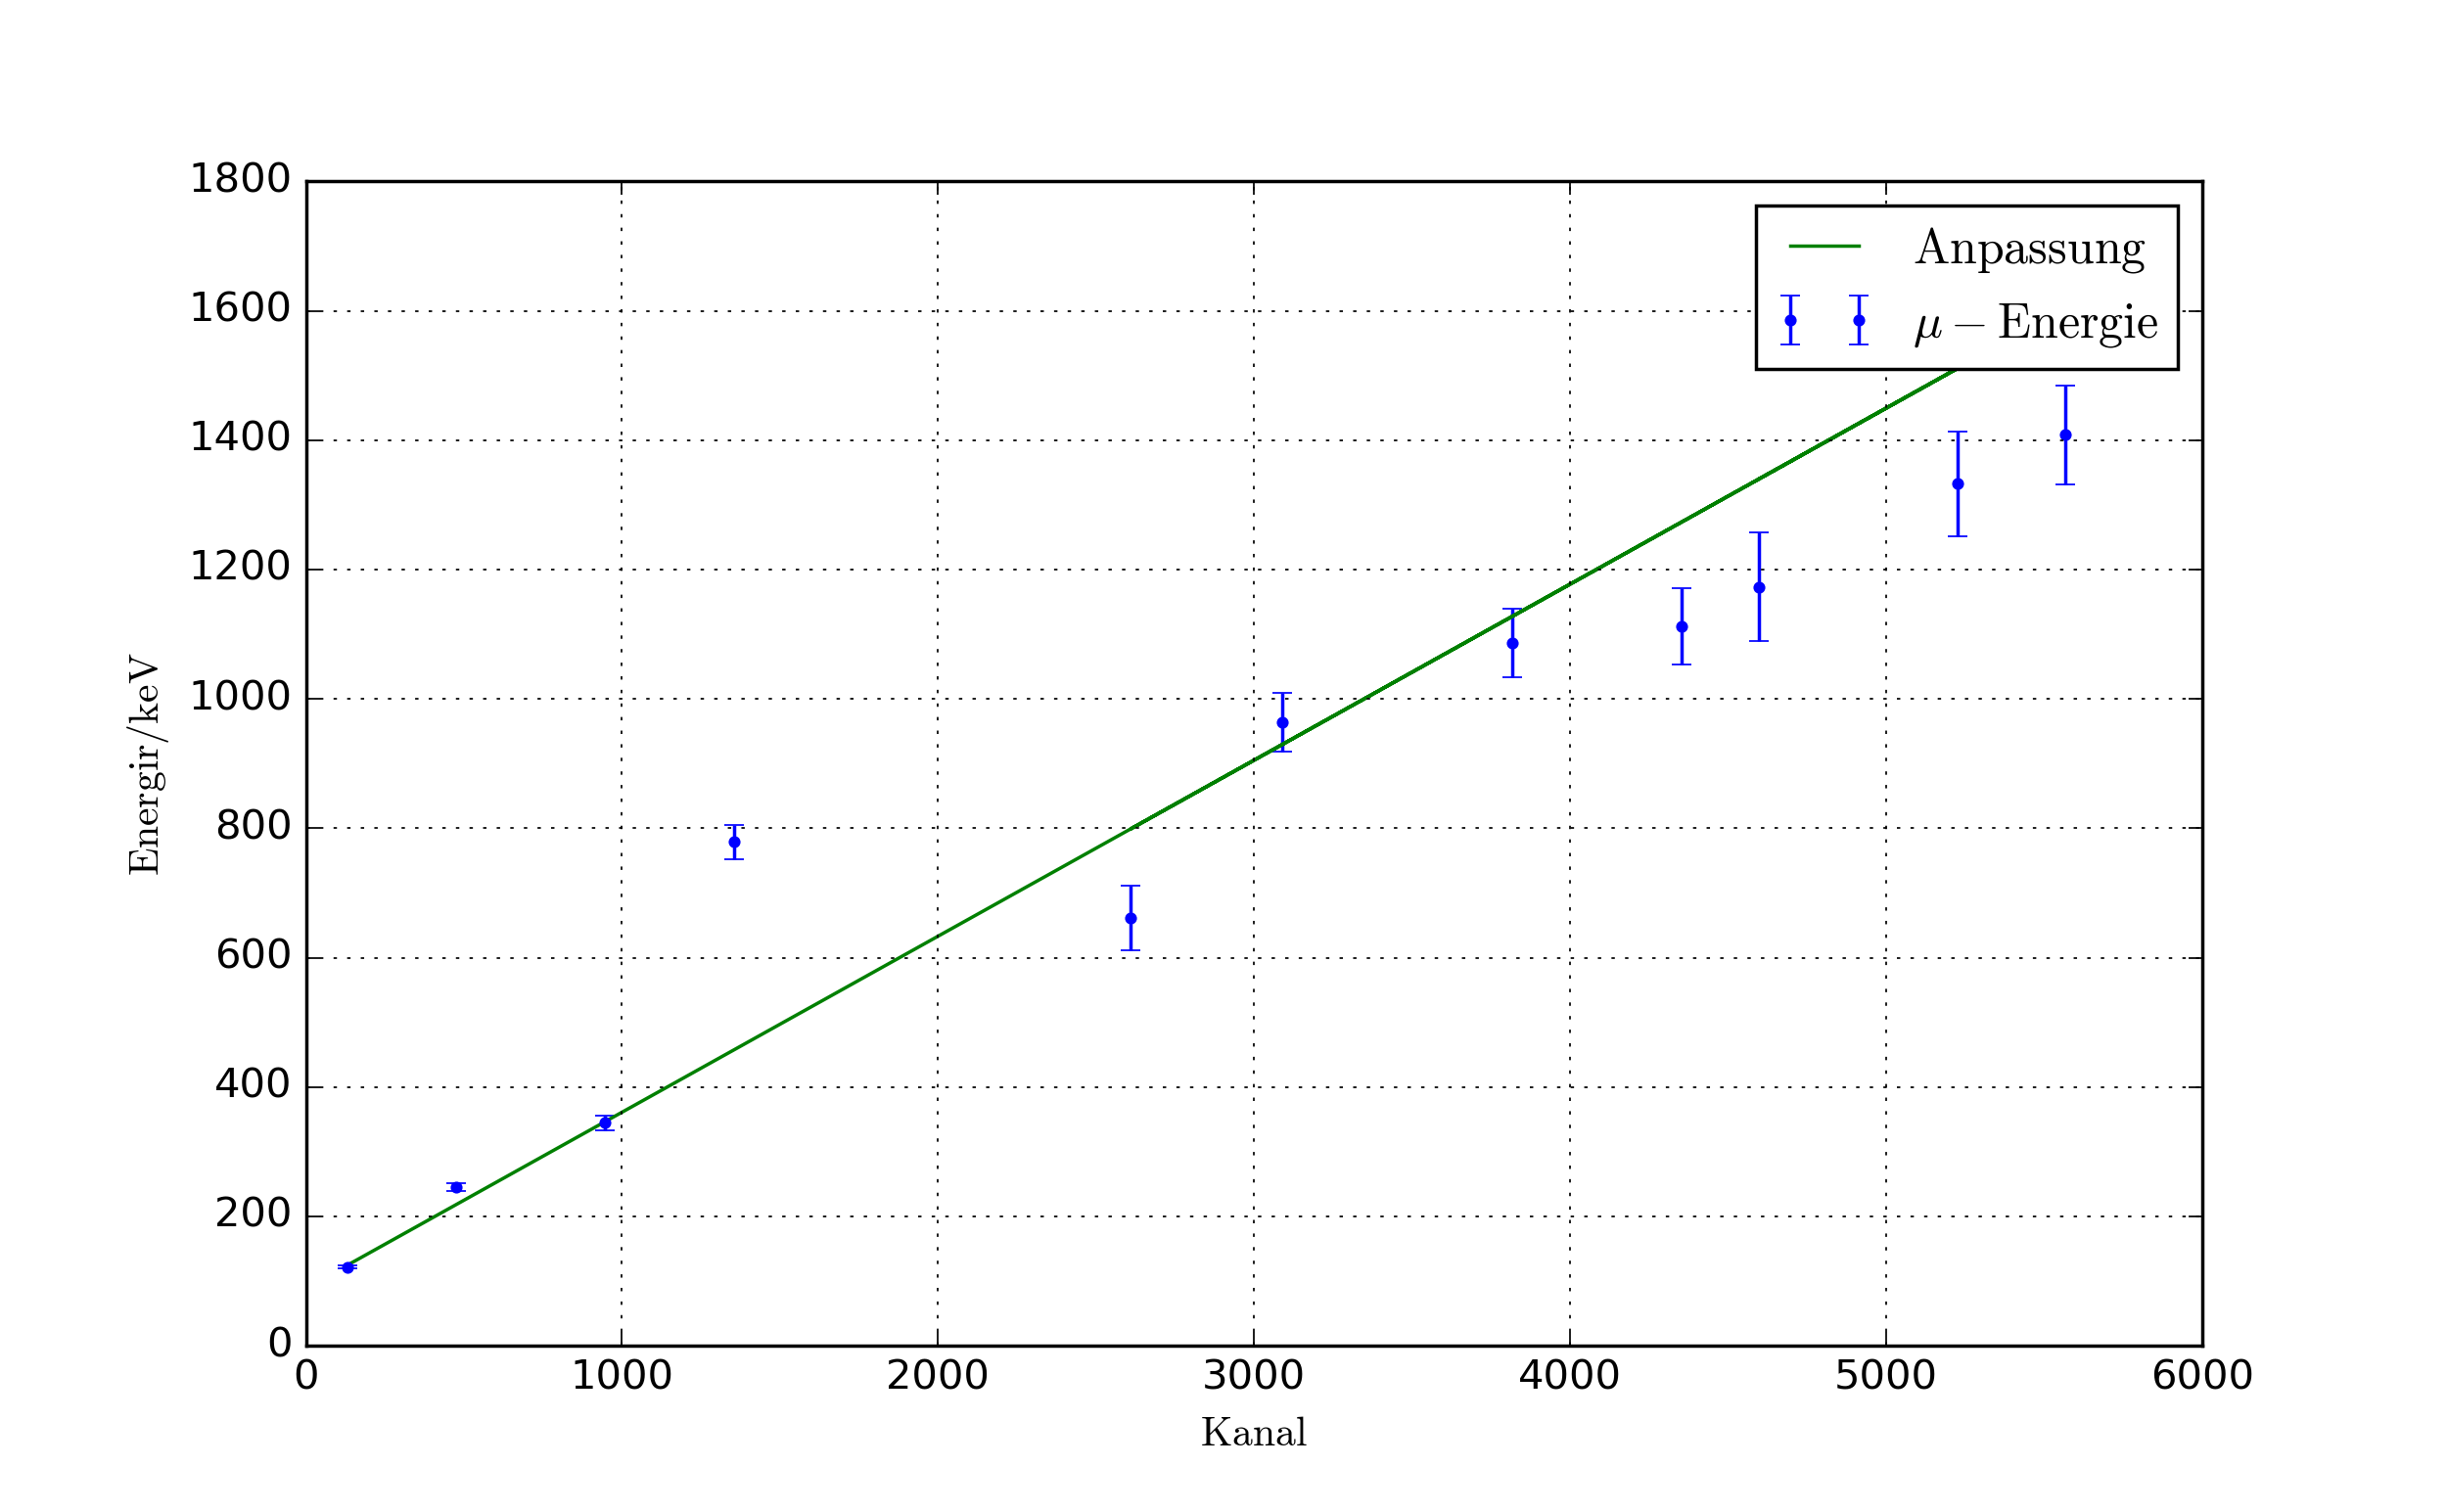
\includegraphics[width=0.45\textwidth]{Szfit.png}
			\caption{Geradenanpassung von Szintillationsdetektor zur Energiekalibration}
			\label{fig:szfit}
		\end{figure}
	\begin{figure}[H]
		\centering
		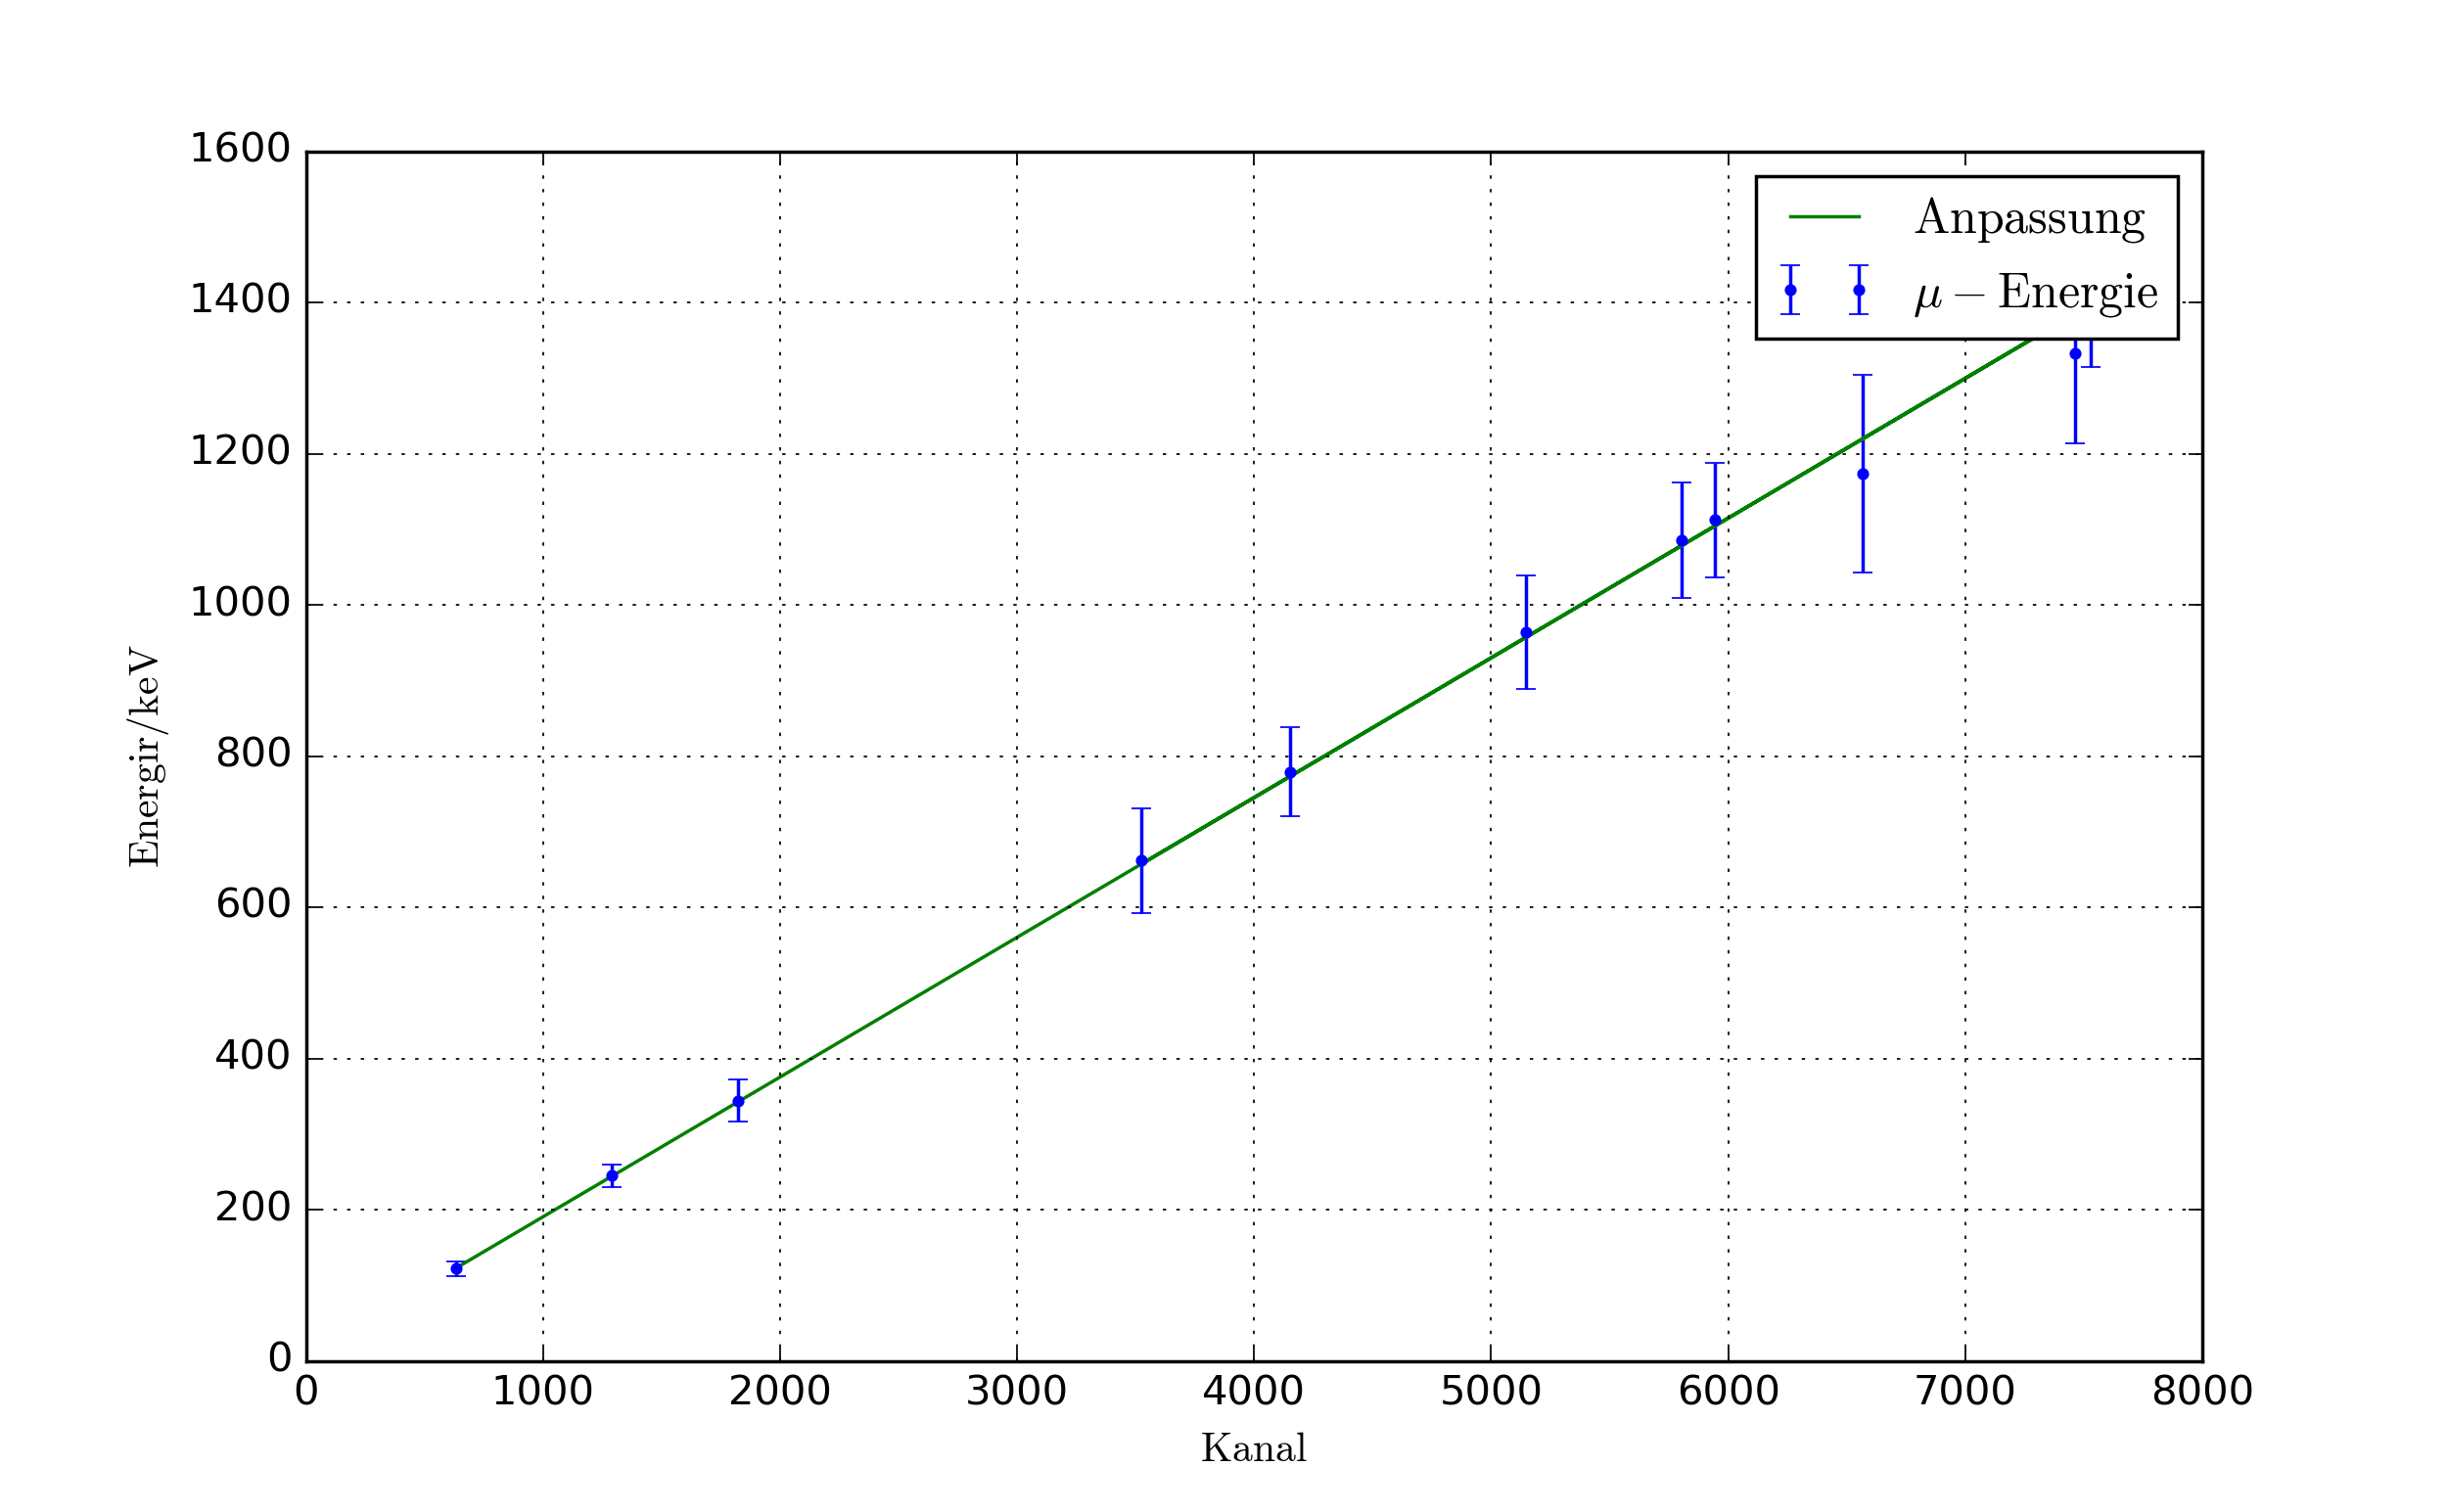
\includegraphics[width=0.45\textwidth]{Gefit.png}
		\caption{Geradenanpassung von Ge-Detektor zur Energiekalibration}
		\label{fig:gefit}
	\end{figure}
	Die Ergebnissen und deren Fehler sind:
	\begin{center}
		\begin{tabular}{|c|c|c|}
			\hline
			Detektor& Szintillator & Halbleiterdetektor\\ \hline
			$a$/(keV/Kanal) & 0.272&0.185\\ \hline
			$\Delta a$/(keV/Kanal) & 0.005&0.006\\ \hline
			$b$/(keV/Kanal) &  88.728 &5.558\\ \hline
			$\Delta b$/(keV/Kanal)&1.998&0.145\\ \hline
		\end{tabular}
	\end{center}
	\subsection{Halbwertsbreite}
	Die Halbwertsbreite kann nach HWHM bestimmen:
	$$ \mathrm{FWHM} = 2\cdot\mathrm{HWHM} $$
	Die Fehlern ist nach Gau\ss-Fehlerfortpflanzen $\Delta\mathrm{FWHM} = 2\cdot\Delta\mathrm{HWHM}$. Aus der Halbwertbreite und der jeweiligen Energie der Linie kann man die Energieaufl\"osung bestimmen:
	$$ \text{Aufl\"osung}=\frac{\mathrm{FWHM}}{E} $$ Die Ergebnissen werden in Tabelle (\ref{tab:auflosung}) dargestellt. Man kann sehen, dass die Aufl\"osungen von Halbleiterdetektor ist deutlich kleiner (immer unter 10\%) als Szintillator (gr\"o\ss er als 20\%).
	\subsection{Intrinsische Halbwertsbreite des Ge-Detektors}
	 Die Halbwertbreite des Halbleiterdetektors ($\Delta E(E_\gamma)$) besteht aus einem intrinsischen und einem elektronischen Anteil ($\Delta E(E_\gamma)$ und $\Delta E_e$, wobei hier $E_\gamma$ ist die Energie des Photons):
	 $$
	 \Delta E(E_\gamma) = \sqrt{ (\Delta E(E_\gamma))^2 + \Delta E_e^2 }
	 $$
	 Der intrinsische Anteil basiert auf den statistischen Prozessen der Ladungssammlung im Ge-Kristall. Deswegen ist es abh\"angig von der Energie des Photons. Die elektronische Anteil basiert auf der Rauschen in elektronische Schaltung. Die theoretische Analyse ergibt eine N\"aherung von intrinsische Anteil:
	 $$ \Delta E(E_\gamma) = \sqrt{c}\cdot\sqrt{E_\gamma} $$
	 wobei $c$ ist eine Konstant.
	 Um diese Zusammenhang zu \"uberpr\"ufung, wir tragen die Quadrat von beide Seit:
	 $$ \Delta E^2 = c\cdot E_\gamma + \Delta E_e^2 $$
	 dann f\"uhren wir eine Geradenanpassung ($E_\gamma$ gegen $\Delta E$), die Steigung ist dann $c$ und $\Delta E_e^2$ ist Abschnitt. Hier benutzen wir  $\Delta E$ und $E_\gamma$ in Einheit von Kanal (dann ist $\Delta E$ FWHM und $E_\gamma$ ist $\mu$) und $\Delta E_e^2$ wird auch in Einheit von Kanal bestimmt. Man kann immer durch Gleichung (\ref{eq: energiekanal}) das Einheit zu keV umwandeln. 
	 \begin{figure}[H]
	 	\centering
	 	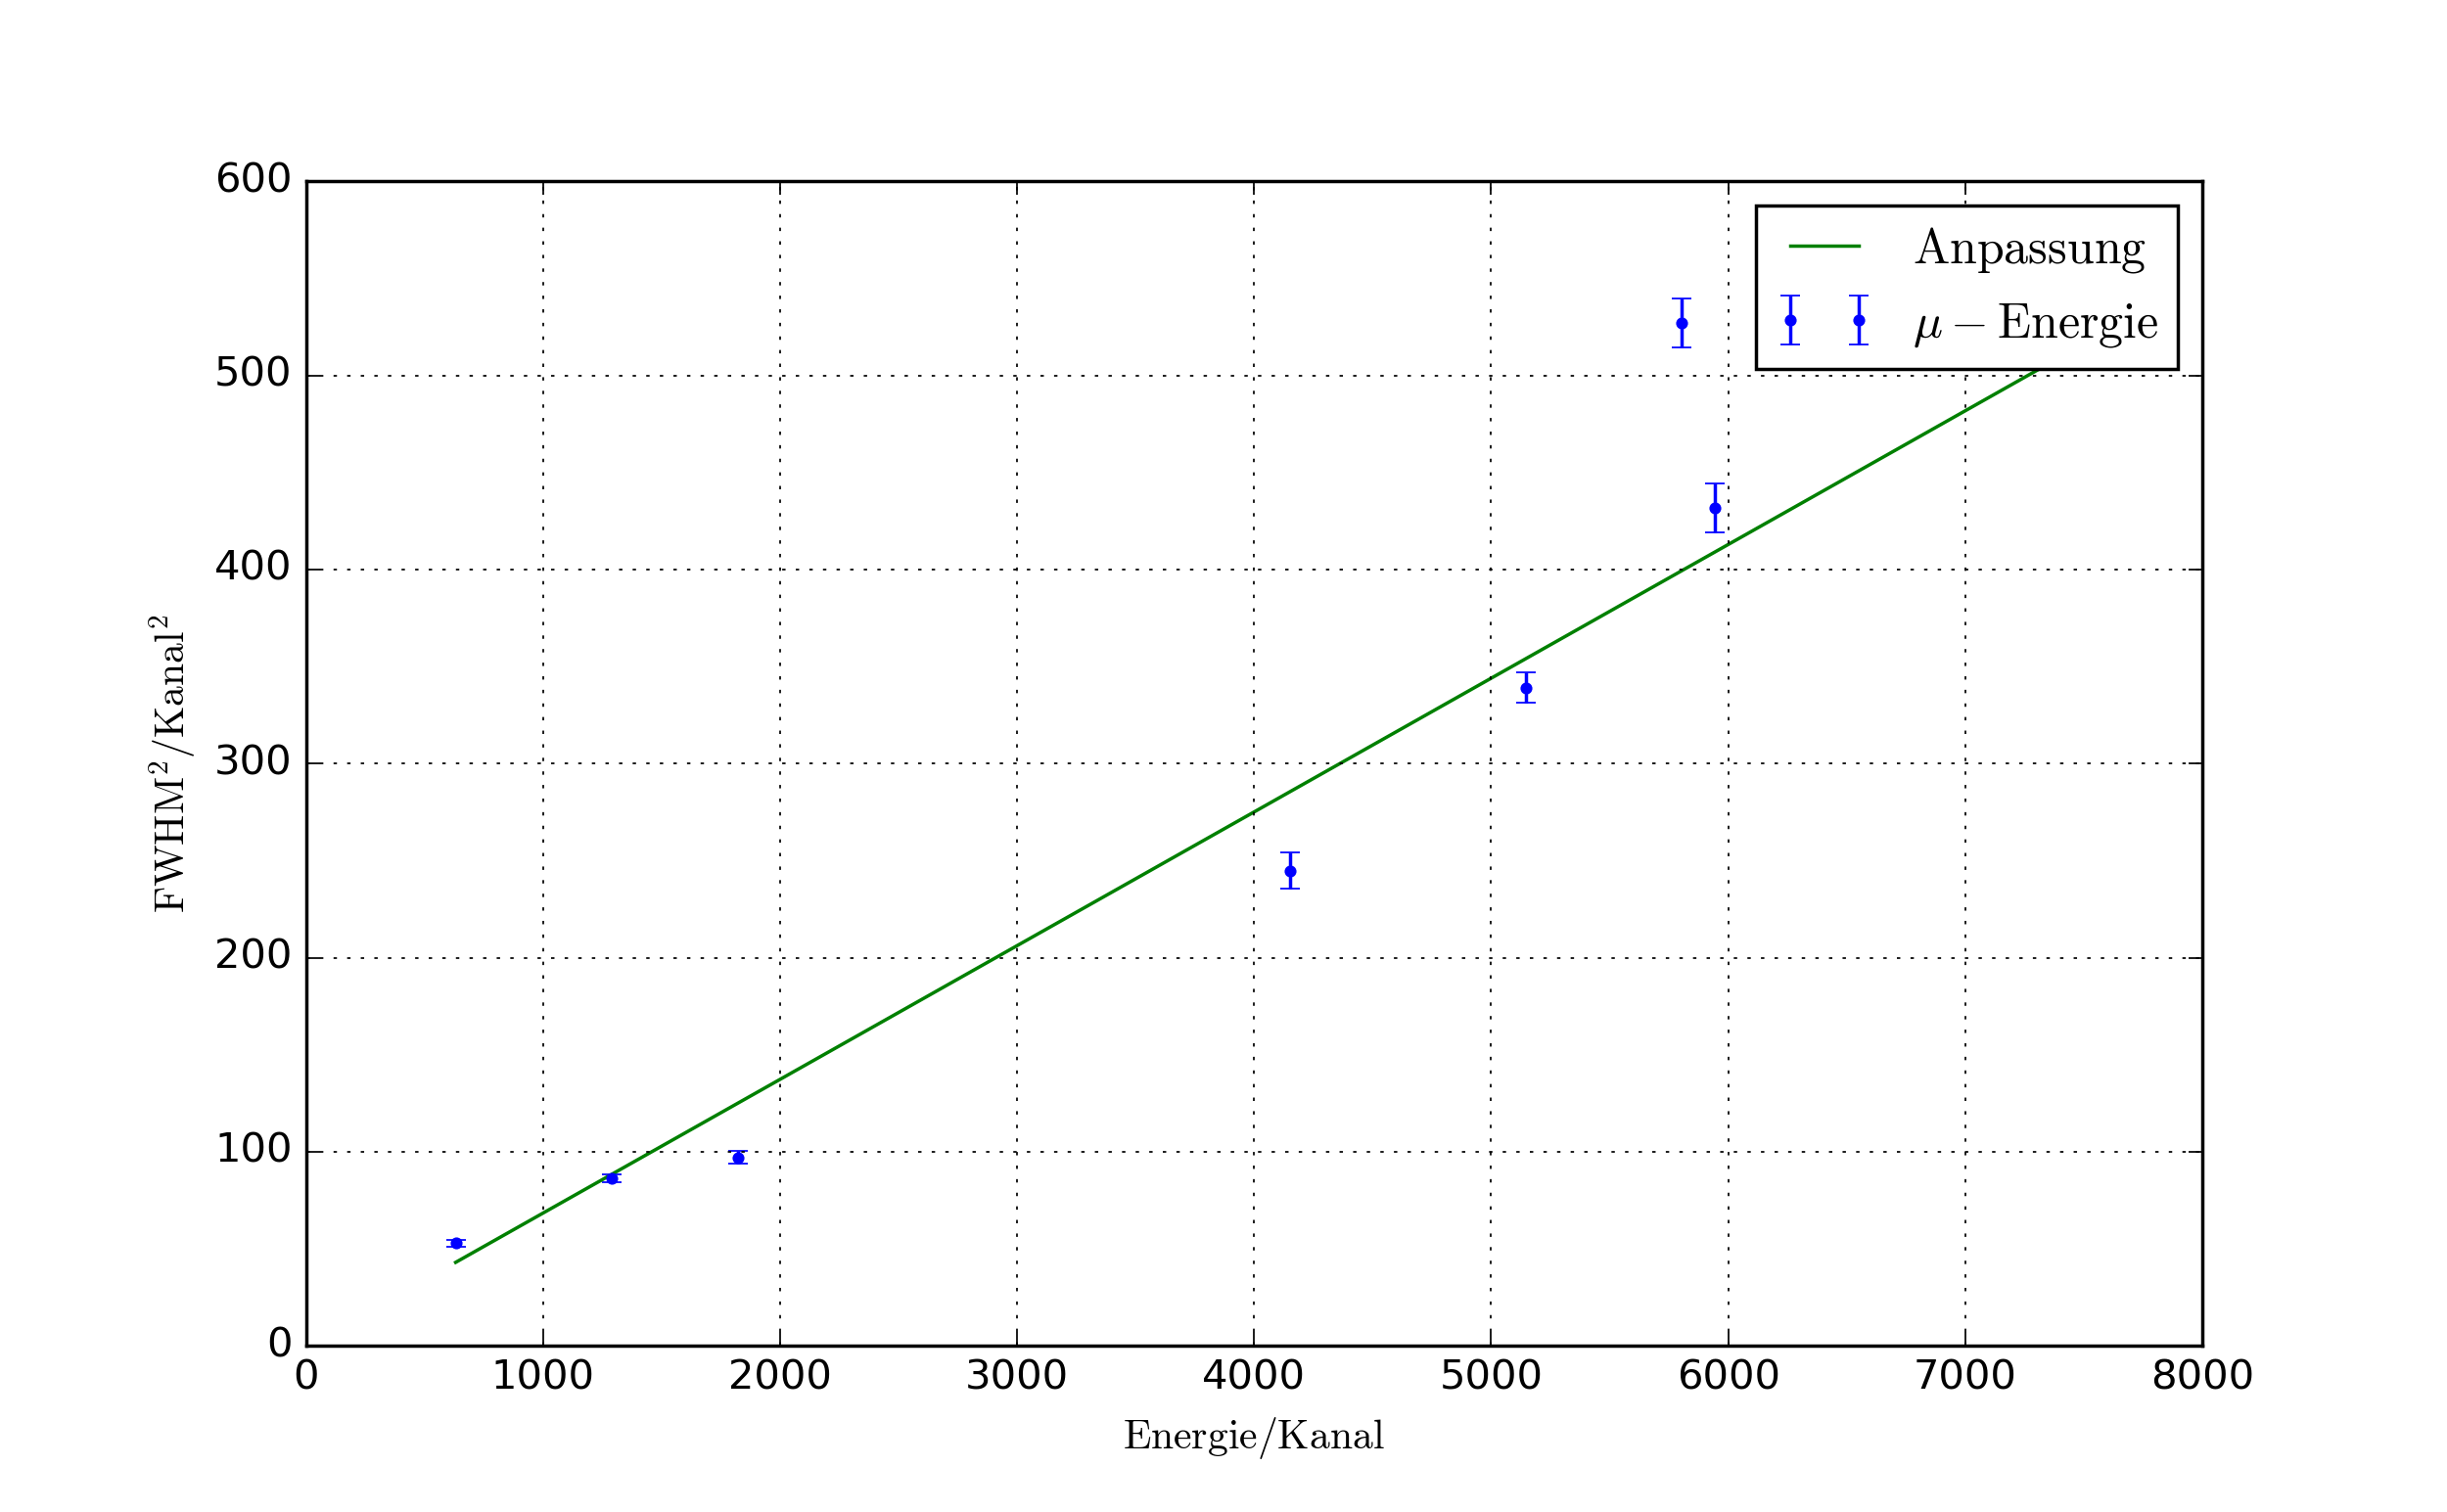
\includegraphics[width=0.45\textwidth]{Halbwertfit.png}
	 	\caption{Quadrat der Halbwertsbreite des Ge-Detektors in Abh\"angigkeit von der Gammaenergie in Einheit Kanal.}
	 	\label{fig:halbwertfit}
	 \end{figure}
 	 Die Ergebnis ist $c = 0,068\pm0,001$ und $\Delta E_e = (-0.607\pm1.881)\mathrm{Kanal}$. Das Fehler von $\Delta E_e$ ist sehr gro\ss. Es kann sein, dass es Rauschen in unsere Messung gibt, oder $\Delta E_e$ hat noch andere Abh\"angigkeit, z.B. von Temperatur oder Verst\"arkung, und diese Parametern ver\"andert wahrend Messung.
	 \subsection{Peak-to-Total-Verh\"altnis}
	 Um das Peak-to-Total-Verh\"altnis zu bestimmen, muss man die Anzahl der im Photopeak registrierten Gammaquanten berechnen nach
	 $$
	 A_{ph} = \sqrt{2*\pi}A\sigma.
	 $$
	 Man muss noch das R\"uckstreuanteil im Niederenergiebereich ber\"ucksichtigen. Dazu wird Gau\ss-Kurve-Anpassung und daraus die Anzahl der Gammaquanten bestimmt. Am Ende kann man das Verh\"altnis berechnen nach:
	 $$
	 PT = \frac{A_{ph}}{N_{tot}-N_{rck}}
	 $$
	 F\"ur Cs wird 663keV-Linie verwendet und f\"ur Co wird die mittlere Energie der beiden Linien (~1250KeV) verwendet. Daraus ergibt sich die Peak-to-Total-Verh\"altnis
	 \begin{center}
	 	\begin{tabular}{|c|c|c|c|}
	 		\hline
	 		Detektor&Element & Peak-to-Total/\% &Fehler/\%\\ \hline
	 		Szintillator& Co & 42.21 & 0.52\\ \hline
	 		Szintillator& Cs & 45.06 & 0.21\\ \hline
	 		Ge-Detektor& Co & 12.11 & 0. 15\\ \hline
	 		Ge-Detektor& Cs & 19.01 & 0.19\\ \hline
	 	\end{tabular}
	 \end{center}
 	Das Peak-to-Total-Verh\"altnis ist f\"ur den Szintillator h\"oher als f\"ur den Halbleiterdetektor. Das Grund daf\"ur ist, dass der Wirkungsquerschnitt proportional zu $Z^5$ ist. F\"ur Ge ist $Z = 32$ und f\"ur Jod(Szintillator) ist $Z = 53$. Wegen die Cs-Linie eine geringe Energie besitzt ist hier der Wirkungsquerschnitt gr\"o\ss er und somit das Peak-to-Total.
	 





























	\end{multicols}
\newpage
\begin{table}
	\centering
	\begin{tabular}{|c|c|c|c|c|c|c|}
		\hline
		Quelle & \multicolumn{2}{|c|}{$^{152}\mathrm{Eu}$}&\multicolumn{2}{|c|}{$^{60}\mathrm{Co}$}&\multicolumn{2}{|c|}{$^{137}\mathrm{Cs}$}\\ \hline
		Detektor& $d$/cm & $t$/s& $d$/cm & $t$/s& $d$/cm & $t$/s\\ \hline
		Szintillator & $5,3\pm0,5$ & $601.059 \pm0.0005$ & $5,5\pm 0,5$ & $613.322\pm0.0005$ & $5,5\pm0,5$ & $600.479 \pm0.0005$\\ \hline
		Halbleiter & $1.5\pm0,5$ & $608.734\pm 0.0005$ & $4,0\pm 0,5$ & $604.075\pm 0.0005$ & $4,5\pm0,5$ &$589.719 \pm 0.0005$ \\ \hline
	\end{tabular}
	\caption{Messung W: Abst\"ande $d$ zwischen Mittelpunkt der Quelle und den Detektoren und die  jeweilligen Messdauern $t$.}
\end{table}
\begin{table}
	\centering
	\begin{tabular}{|c|c|c|c|c|c|c|}
		\hline
		Quelle & \multicolumn{2}{|c|}{$^{152}\mathrm{Eu}$}&\multicolumn{2}{|c|}{$^{60}\mathrm{Co}$}&\multicolumn{2}{|c|}{$^{137}\mathrm{Cs}$}\\ \hline
		Detektor& $d$/cm & $t$/s& $d$/cm & $t$/s& $d$/cm & $t$/s\\ \hline
		Szintillator & $5,3\pm0,5$ & & $5,5\pm 0,5$ & & $5,5\pm0,5$ & \\ \hline
		Halbleiter & $1.5\pm0,5$ & & $4,0\pm 0,5$ & & $4,5\pm0,5$ & \\ \hline
	\end{tabular}
	\caption{Messung L: Abst\"ande $d$ zwischen Mittelpunkt der Quelle und den Detektoren und die jeweilligen Messdauern $t$.}
\end{table}
\begin{table}[htbp]
	\centering
	\begin{tabular}{|l|r|r|r|r|r|r|r|}
		\hline
		Element & {Energie/keV} & {$A$} & {$\Delta A$} & {$\mu$} &{$\Delta mu$} & {$\sigma$} & \multicolumn{1}{l}{$\Delta \sigma$} \\\hline
		Co      & 1173.2                          & 3084.807                & 100.381                        & 6567.571                  & 78.482                          & 6.62                         & 0.126                               \\\hline
		Co      & 1332.5                          & 2500.892                & 99.776                         & 7462.482                  & 91.305                          & 7.147                        & 0.106                               \\\hline
		Cs      & 661.7                           & 56518.83                & 2021.929                       & 3524.197                  & 68.452                          & 6.808                        & 0.075                               \\\hline
		Eu      & 1408                            & 4025.367                & 130.023                        & 7530.873                  & 103.757                         & 11.863                       & 0.122                               \\\hline
		Eu      & 1112.1                          & 4039.113                & 121.73                         & 5941.807                  & 73.945                          & 10.389                       & 0.162                               \\\hline
		Eu      & 1085.9                          & 3141.106                & 118.467                        & 5801.954                  & 99.248                          & 11.48                        & 0.139                               \\\hline
		Eu      & 964.1                           & 5358.213                & 198.316                        & 5147.464                  & 95.308                          & 9.207                        & 0.092                               \\\hline
		Eu      & 778.9                           & 6862.642                & 250.076                        & 4153.157                  & 60.589                          & 7.823                        & 0.086                               \\ \hline
		Eu      & 344.3                           & 45676.31                & 1418.568                       & 1823.311                  & 28.749                          & 4.925                        & 0.083                               \\ \hline
		Eu      & 244.7                           & 20574.34                & 750.483                        & 1290.334                  & 16.082                          & 4.648                        & 0.061                               \\ \hline
		Eu      & 121.8                           & 122673.8                & 4291.804                       & 631.824                   & 11.704                          & 3.631                        & 0.038                           \\ \hline   
	\end{tabular}
	\caption{Ergebnis von Gau\ss-Kurven-Anpassung f\"ur die Spektren des Halbleiterdetektors.}
	\label{tab:gefit}
\end{table}
\begin{table}[htbp]
	\centering
	\begin{tabular}{|l|r|r|r|r|r|r|r|}
		\hline
		Element &
		{Energie/keV} &
		{$A$} &
		{$\Delta A$} &
		{$\mu$} &
		{$\Delta mu$} &
		{$\sigma$} &
		{$\Delta \sigma$} \\ \hline
		Co & 1173.2 & 97.334   & 3.353    & 4597.38  & 50.158 & 150.74  & 2.604 \\ \hline
		Co & 1332.5 & 76.43    & 2.644    & 5225.95  & 65.186 & 147.238 & 1.678 \\ \hline
		Cs & 661.7  & 3376.521 & 134.099  & 2608.751 & 34.898 & 103.564 & 1.649 \\ \hline
		Eu & 1112.1 & 780.083  & 26.87    & 4352.501 & 85.235 & 179.351 & 1.829 \\ \hline
		Eu & 1408   & 373.767  & 12.565   & 5566.75  & 82.859 & 164.062 & 2.47  \\ \hline
		Eu & 1085.9 & 676.632  & 25.912   & 3816.279 & 47.024 & 166.179 & 1.723 \\ \hline
		Eu & 964.1  & 1014.79  & 35.044   & 3088.018 & 54.518 & 156.29  & 1.841 \\ \hline
		Eu & 778.9  & 5993.97  & 189.316  & 1355.607 & 14.089 & 87.869  & 1.309 \\ \hline
		Eu & 344.3  & 4679.29  & 172.217  & 947.093  & 11.884 & 78.436  & 0.794 \\ \hline
		Eu & 244.7  & 26858.79 & 891.59   & 474.656  & 6.97   & 32.993  & 0.403 \\ \hline
		Eu & 121.8  & 59778.7  & 2142.021 & 132.717  & 2.442  & 21.546  & 0.239 \\ \hline
	\end{tabular}
	\caption{Ergebnis von Gau\ss-Kurven-Anpassung f\"ur die Spektren des Szintillationsdetektros.}
	\label{tab:szfit}
\end{table}
\begin{figure}[htbp]
	\centering
	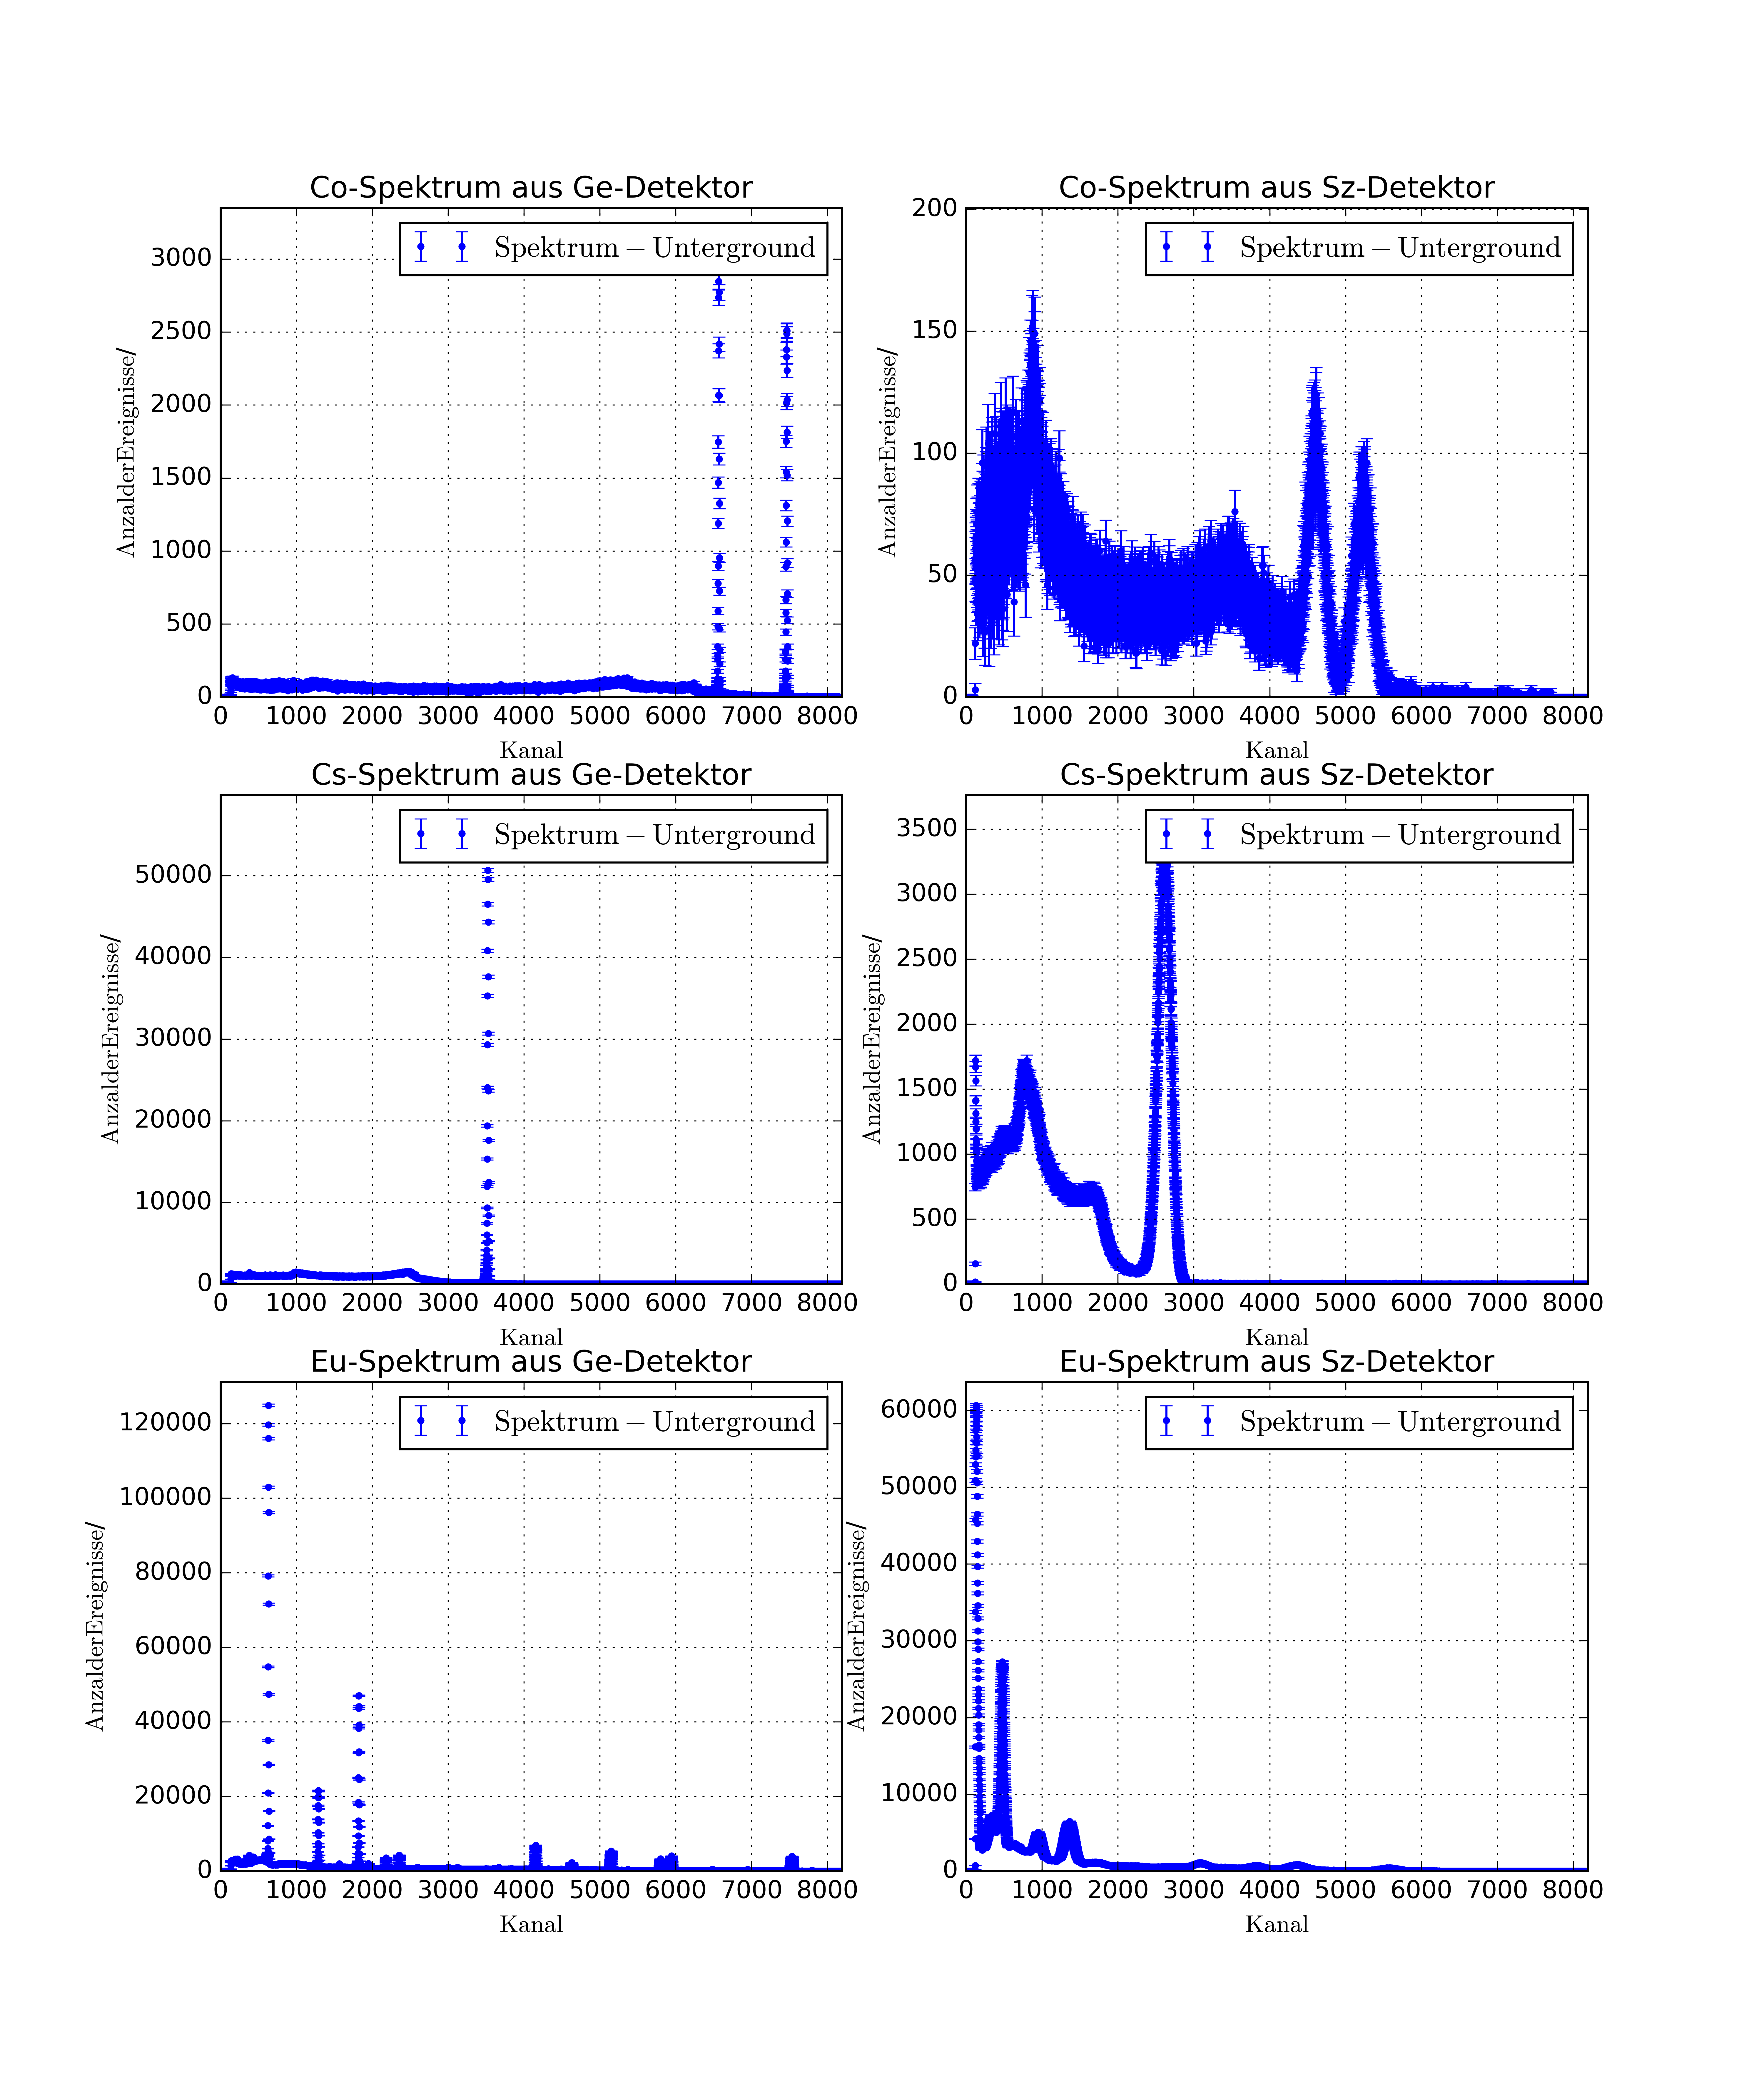
\includegraphics[width=\textwidth]{spektrumminusunter.png}
	\caption{Spektren ohne Untergrunde}
	\label{fig:spektrummunusunter}
\end{figure}
\begin{table}[htbp]
	\centering
	\begin{tabular}{|c|c|c|c|c|}
		\hline
		&
		\multicolumn{2}{c|}{Szintillator} &
		\multicolumn{2}{c|}{Halbleiterdetektor} \\ \hline
		& {Aufl"osung/\%} &
		{$\Delta$Aufl"osung/\%} &
		{Aufl"osung/\%} &
		{$\Delta$Aufl"osung/\%} \\ \hline
		Co & 25.7  & 0.47 & 1.13 & 0.02 \\ \hline
		Co & 22.1  & 0.3  & 1.07 & 0.02 \\ \hline
		Cs & 31.3  & 0.45 & 2.06 & 0.04 \\ \hline
		Eu & 32.25 & 0.51 & 1.69 & 0.02 \\ \hline
		Eu & 23.3  & 0.34 & 1.87 & 0.02 \\ \hline
		Eu & 30.61 & 0.42 & 2.11 & 0.03 \\ \hline
		Eu & 32.42 & 0.63 & 1.91 & 0.03 \\ \hline
		Eu & 22.56 & 0.4  & 2.01 & 0.02 \\ \hline
		Eu & 45.56 & 0.69 & 2.86 & 0.04 \\ \hline
		Eu & 26.97 & 0.4  & 3.8  & 0.04 \\ \hline
		Eu & 35.38 & 0.42 & 5.96 & 0.06 \\ \hline
	\end{tabular}
\caption{Energieaufl\"osung. Hier wird die Halbwertsbreten nicht dargestellt, da man einfach aus HWHM berechnen kann.}
\label{tab:auflosung}
\end{table}
\newpage
\begin{thebibliography}{9}

	\bibitem[detektor]{detektor} Kleinknecht, Konrad, \textit{Detektoren für Teilchenstrahlung}, B.G. Teubnerer Stuttgart, 1992, 19ff.

	\bibitem[techniques]{techniques} Leo, W.R., \textit{Techniques for Nuclear and Particle Physics Experiments}, Springer Verlag, 1994, 113, 157ff.,177ff.,192, 204ff., 313f.

	\bibitem[gerthsen]{gerthsen} Meschede, D., \textit{Gerthsen Physik}, Springer Verlag, 2004, 464-465,672-673,841

	\bibitem[messelektronik]{messelektronik} Schmidt, H.U., \textit{Meßelektronik in der Kernphysik}, Teubner Verlag, 1986, 21,28,38,79-80,106-107,110,119-120,184-185

	\bibitem[teilchen]{teilchen} Kolanoski, H., \textit{Teilchendetektoren: Grundlagen und Anwendungen}, Springer Spektrum, 2016, 524

	\bibitem[kern]{kern} Amsler, Claude, \textit{Kern- und Teilchenphysik}, Zürich: Vdf-Hochschulverl., 2007, 238
\end{thebibliography}

%\nocite{*}
%\printbibliography		
\end{document}
